\documentclass[11pt,a4paper]{report}
\usepackage[textwidth=37em,vmargin=30mm]{geometry}
\usepackage{calc,xunicode,amsmath,amssymb,paralist,enumitem,tabu,booktabs,datetime2,xeCJK,xeCJKfntef,listings}
\usepackage{tocloft,fancyhdr,tcolorbox,xcolor,graphicx,eso-pic,xltxtra,xelatexemoji}

\newcommand{\envyear}[0]{2025}
\newcommand{\envdatestr}[0]{2025-01-21}
\newcommand{\envfinaldir}[0]{webdb/2025/20250121/final}

\usepackage[hidelinks]{hyperref}
\hypersetup{
    colorlinks=false,
    pdfpagemode=FullScreen,
    pdftitle={Web Digest - \envdatestr}
}

\setlength{\cftbeforechapskip}{10pt}
\renewcommand{\cftchapfont}{\rmfamily\bfseries\large\raggedright}
\setlength{\cftbeforesecskip}{2pt}
\renewcommand{\cftsecfont}{\sffamily\small\raggedright}

\setdefaultleftmargin{2em}{2em}{1em}{1em}{1em}{1em}

\usepackage{xeCJK,xeCJKfntef}
\xeCJKsetup{PunctStyle=plain,RubberPunctSkip=false,CJKglue=\strut\hskip 0pt plus 0.1em minus 0.05em,CJKecglue=\strut\hskip 0.22em plus 0.2em}
\XeTeXlinebreaklocale "zh"
\XeTeXlinebreakskip = 0pt


\setmainfont{Brygada 1918}
\setromanfont{Brygada 1918}
\setsansfont{IBM Plex Sans}
\setmonofont{JetBrains Mono NL}
\setCJKmainfont{Noto Serif CJK SC}
\setCJKromanfont{Noto Serif CJK SC}
\setCJKsansfont{Noto Sans CJK SC}
\setCJKmonofont{Noto Sans CJK SC}

\setlength{\parindent}{0pt}
\setlength{\parskip}{8pt}
\linespread{1.15}

\lstset{
	basicstyle=\ttfamily\footnotesize,
	numbersep=5pt,
	backgroundcolor=\color{black!5},
	showspaces=false,
	showstringspaces=false,
	showtabs=false,
	tabsize=2,
	captionpos=b,
	breaklines=true,
	breakatwhitespace=true,
	breakautoindent=true,
	linewidth=\textwidth
}






\newcommand{\coverpic}[2]{
    % argv: itemurl, authorname
    Cover photo by #2~~(\href{#1}{#1})
}
\newcommand{\makeheader}[0]{
    \begin{titlepage}
        % \newgeometry{hmargin=15mm,tmargin=21mm,bmargin=12mm}
        \begin{center}
            
            \rmfamily\scshape
            \fontspec{BaskervilleF}
            \fontspec{Old Standard}
            \fontsize{59pt}{70pt}\selectfont
            WEB\hfill DIGEST
            
            \vfill
            % \vskip 30pt
            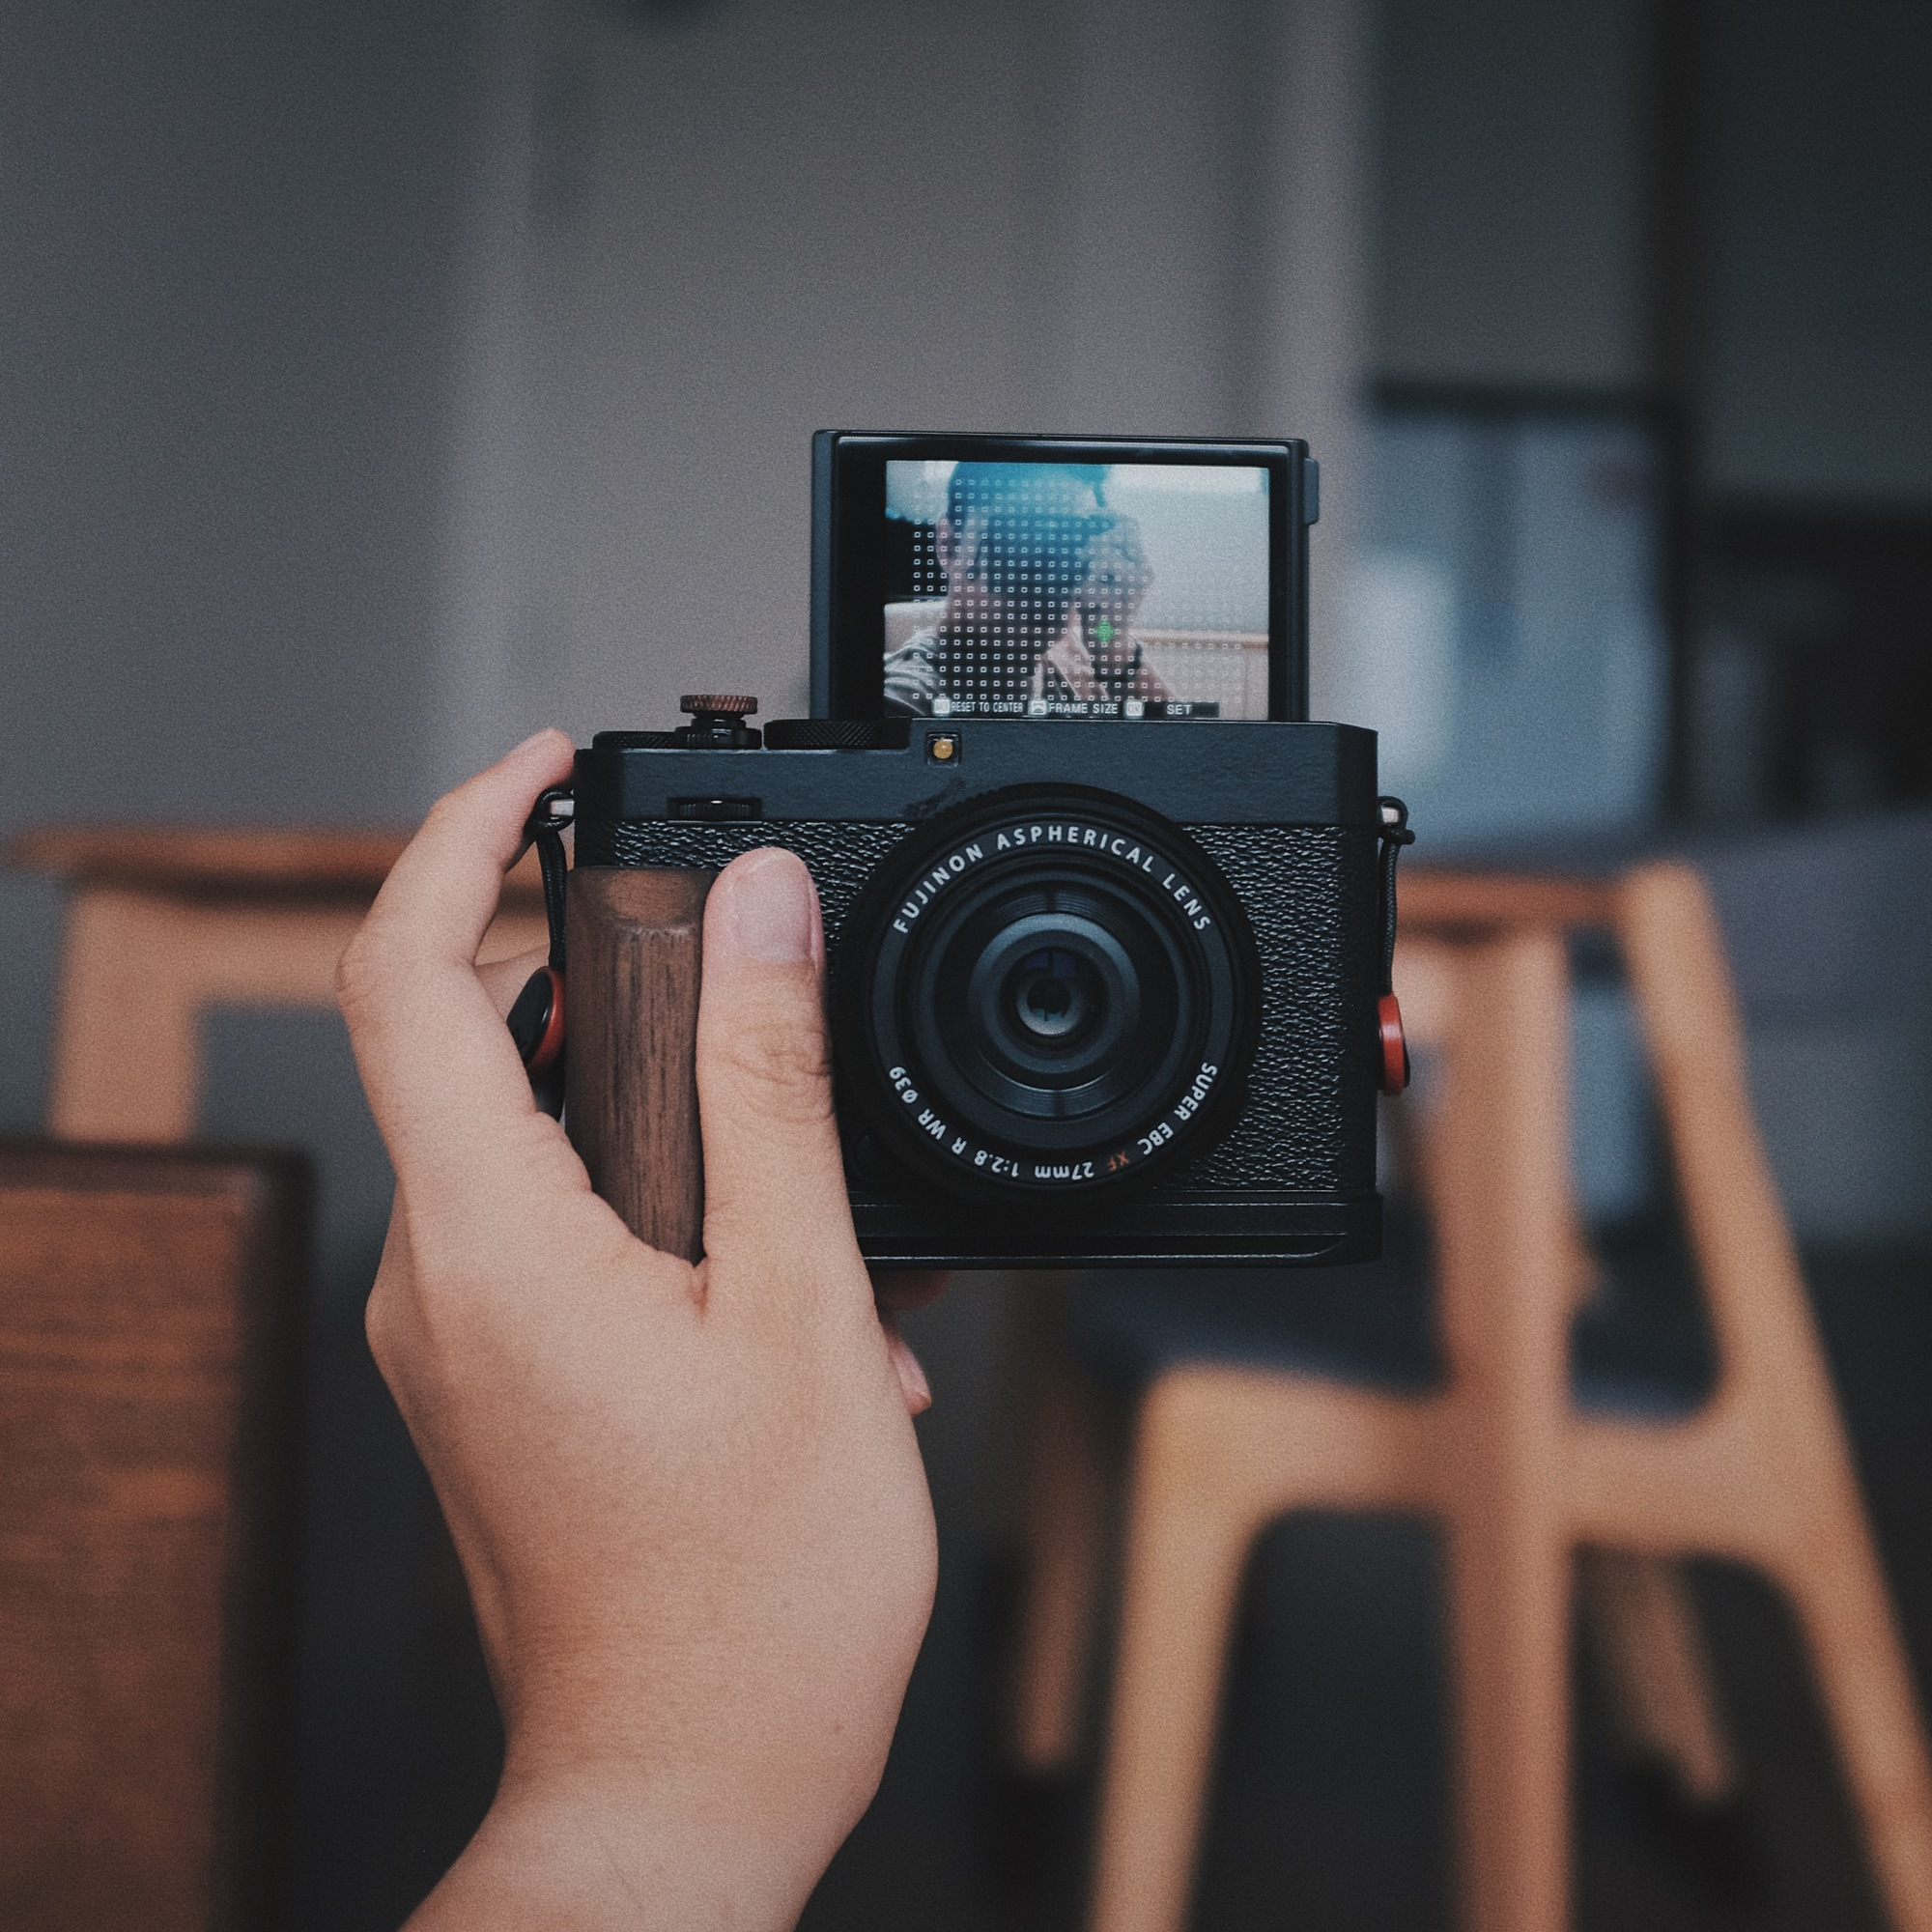
\includegraphics[width=\linewidth]{\envfinaldir/coverpic-prod.jpg}\par
            % \vskip 30pt
            \vfill

            \normalsize\rmfamily\scshape
            \copyright{} The Web Digest Project \hfill\large \envdatestr
        \end{center}
    \end{titlepage}
    % \restoregeometry
}
\newcommand{\simplehref}[1]{%
    \textcolor{blue!80!green}{\href{#1}{#1}}%
}
\renewcommand{\contentsname}{\center\Huge\sffamily\bfseries Contents\par\vskip 20pt}
\newcounter{ipartcounter}
\setcounter{ipartcounter}{0}
\newcommand{\ipart}[1]{
    % \vskip 20pt
    \clearpage
    \stepcounter{ipartcounter}
    \phantomsection
    \addcontentsline{toc}{chapter}{#1}
    % \begin{center}
    %     \Huge
    %     \sffamily\bfseries
    %     #1
    % \end{center}
    % \vskip 20pt plus 7pt
}
\newcounter{ichaptercounter}
\setcounter{ichaptercounter}{0}
\newcommand{\ichapter}[1]{
    % \vskip 20pt
    \clearpage
    \stepcounter{ichaptercounter}
    \phantomsection
    \addcontentsline{toc}{section}{\numberline{\arabic{ichaptercounter}}#1}
    \begin{center}
        \Huge
        \sffamily\bfseries
        #1
    \end{center}
    \vskip 20pt plus 7pt
}
\newcommand{\entrytitlefont}[1]{\subsection*{\raggedright\Large\sffamily\bfseries#1}}
\newcommand{\entryitemGeneric}[2]{
    % argv: title, url
    \parbox{\linewidth}{
        \entrytitlefont{#1}\par\vskip 5pt
        \footnotesize\ttfamily\mdseries
        \simplehref{#2}
    }\vskip 11pt plus 11pt minus 1pt
}
\newcommand{\entryitemGithub}[3]{
    % argv: title, url, desc
    \parbox{\linewidth}{
        \entrytitlefont{#1}\par\vskip 5pt
        \footnotesize\ttfamily\mdseries
        \simplehref{#2}\par\vskip 5pt
        \small\rmfamily\mdseries#3
    }\vskip 11pt plus 11pt minus 1pt
}
\newcommand{\entryitemAp}[3]{
    % argv: title, url, desc
    \parbox{\linewidth}{
        \entrytitlefont{#1}\par\vskip 5pt
        \footnotesize\ttfamily\mdseries
        \simplehref{#2}\par\vskip 5pt
        \small\rmfamily\mdseries#3
    }\vskip 11pt plus 11pt minus 1pt
}
\newcommand{\entryitemHackernews}[3]{
    % argv: title, hnurl, rawurl
    % \parbox{\linewidth}{
    %     \entrytitlefont{#1}\par\vskip 5pt
    %     \footnotesize\ttfamily\mdseries
    %     \simplehref{#3}\par
    %     \textcolor{black!50}{\href{#2}{#2}}
    % }\vskip 11pt plus 11pt minus 1pt
    \begin{minipage}{\linewidth}
            \entrytitlefont{#1}\par\vskip 5pt
            \footnotesize\ttfamily\mdseries
            \simplehref{#3}\par
            \textcolor{black!50}{\href{#2}{#2}}
    \end{minipage}\par\vskip 11pt plus 11pt minus 1pt
}







\begin{document}

\makeheader

\tableofcontents\clearpage




\ipart{Developers}
\ichapter{Hacker News}
\entryitemTwoLinks{Elon Musk appears to make back-to-back fascist salutes at inauguration rally}{https://news.ycombinator.com/item?id=42773778}{https://www.theguardian.com/technology/2025/jan/20/trump-elon-musk-salute}

\entryitemTwoLinks{Did Elon Musk Appear to Sieg Heil at Trump Inauguration?}{https://news.ycombinator.com/item?id=42772995}{https://www.jpost.com/international/article-838444}

\entryitemTwoLinks{ROCm Device Support Wishlist}{https://news.ycombinator.com/item?id=42772170}{https://github.com/ROCm/ROCm/discussions/4276}

\entryitemTwoLinks{I am (not) a failure: Lessons learned from six failed startup attempts}{https://news.ycombinator.com/item?id=42771676}{http://blog.rongarret.info/2025/01/i-am-not-failure-lessons-learned-from.html}

\entryitemTwoLinks{I'm Peter Roberts, immigration attorney, who does work for YC and startups. AMA}{https://news.ycombinator.com/item?id=42770125}{https://news.ycombinator.com/item?id=42770125}

\entryitemTwoLinks{Mixxx: GPL DJ Software}{https://news.ycombinator.com/item?id=42769871}{https://mixxx.org/}

\entryitemTwoLinks{DeepSeek-R1}{https://news.ycombinator.com/item?id=42768072}{https://github.com/deepseek-ai/DeepSeek-R1}

\entryitemTwoLinks{Celestial Navigation for Drones}{https://news.ycombinator.com/item?id=42767797}{https://www.mdpi.com/2504-446X/8/11/652}

\entryitemTwoLinks{Using eSIMs with devices that only have a physical SIM slot via a 9eSIM SIM car}{https://news.ycombinator.com/item?id=42767584}{https://neilzone.co.uk/2025/01/using-esims-with-devices-that-only-have-a-physical-sim-slot-via-a-9esim-sim-card-with-android-and-linux/}

\entryitemTwoLinks{I Met Paul Graham Once}{https://news.ycombinator.com/item?id=42767507}{http://okayfail.com/2025/i-met-pg-once.html}

\entryitemTwoLinks{Zork: The Great Inner Workings (2020)}{https://news.ycombinator.com/item?id=42767132}{https://medium.com/swlh/zork-the-great-inner-workings-b68012952bdc}

\entryitemTwoLinks{TypeScript enums: use cases and alternatives}{https://news.ycombinator.com/item?id=42766729}{https://2ality.com/2025/01/typescript-enum-patterns.html}

\entryitemTwoLinks{Parinfer: Simpler Lisp Editing}{https://news.ycombinator.com/item?id=42766205}{https://shaunlebron.github.io/parinfer/}

\entryitemTwoLinks{What does "supports DRM and may not be fully accessible" mean for SATA SDDs?}{https://news.ycombinator.com/item?id=42765480}{https://unix.stackexchange.com/questions/789838/what-does-supports-drm-functions-and-may-not-be-fully-accessible-mean-for-sata}

\entryitemTwoLinks{I'll think twice before using GitHub Actions again}{https://news.ycombinator.com/item?id=42764762}{https://ninkovic.dev/blog/2025/think-twice-before-using-github-actions}

\entryitemTwoLinks{Reverse Engineering Bambu Connect}{https://news.ycombinator.com/item?id=42764602}{https://wiki.rossmanngroup.com/wiki/Reverse\_Engineering\_Bambu\_Connect}

\entryitemTwoLinks{Ask HN: Is anyone making money selling traditional downloadable software?}{https://news.ycombinator.com/item?id=42764185}{https://news.ycombinator.com/item?id=42764185}

\entryitemTwoLinks{UK's hardware talent is being wasted}{https://news.ycombinator.com/item?id=42763386}{https://josef.cn/blog/uk-talent}

\entryitemTwoLinks{FrontierMath was funded by OpenAI}{https://news.ycombinator.com/item?id=42763231}{https://www.lesswrong.com/posts/cu2E8wgmbdZbqeWqb/meemi-s-shortform}

\entryitemTwoLinks{It's time to make computing personal again}{https://news.ycombinator.com/item?id=42763095}{https://www.vintagecomputing.com/index.php/archives/3292/the-pc-is-dead-its-time-to-make-computing-personal-again}\ichapter{Phoronix}
\entryitemGeneric{\hskip 0pt{}AMD Seeking Feedback Around What Radeon GPUs You Would Like Supported By ROCm}{https://www.phoronix.com/news/AMD-Feedback-ROCm-Support}

\entryitemGeneric{\hskip 0pt{}Wine 10.0 Expected This Week For Improving Windows Software On Linux}{https://www.phoronix.com/news/Wine-10.0-Features}

\entryitemGeneric{\hskip 0pt{}Bcachefs Sends In "The Last Big On Disk Format Upgrade" For Linux 6.14}{https://www.phoronix.com/news/Bcachefs-Linux-6.14}

\entryitemGeneric{\hskip 0pt{}RADV Vulkan Driver Support Being Worked On For The GPU Found In The Sony PS5 \& BC-250}{https://www.phoronix.com/news/AMD-RADV-PS5-BC-250}

\entryitemGeneric{\hskip 0pt{}NVIDIA GeForce RTX 5090 Arrives For Linux Testing}{https://www.phoronix.com/review/nvidia-geforce-rtx-5090-pre}

\entryitemGeneric{\hskip 0pt{}Linux 6.14 To Allow VirtualBox Guest Support On ARM64 VMs}{https://www.phoronix.com/news/Linux-6.14-VirtualBox-Guest-ARM}

\entryitemGeneric{\hskip 0pt{}More Rust Code Is Coming For Linux 6.14 Along With Hitting Another "Major Milestone"}{https://www.phoronix.com/news/Linux-6.14-Rust}

\entryitemGeneric{\hskip 0pt{}Intel FFmpeg Cartwheel 2024Q4 Adds Battlemage GPU Support}{https://www.phoronix.com/news/Intel-FFmpeg-2024Q4-Battlemage}

\entryitemGeneric{\hskip 0pt{}Many Scheduler Improvements Ready To Better Enhance The Linux 6.14 Kernel}{https://www.phoronix.com/news/Linux-6.14-Scheduler}\ichapter{Dribbble}
\entryitemGeneric{\hskip 0pt{}Monocle Cat}{https://dribbble.com/shots/25502155-Monocle-Cat}

\entryitemGeneric{\hskip 0pt{}Personal Banking App}{https://dribbble.com/shots/25493958-Personal-Banking-App}

\entryitemGeneric{\hskip 0pt{}404}{https://dribbble.com/shots/25492419-404}

\entryitemGeneric{\hskip 0pt{}Wine Label}{https://dribbble.com/shots/25490604-Wine-Label}

\entryitemGeneric{\hskip 0pt{}planet}{https://dribbble.com/shots/25490310-planet}

\entryitemGeneric{\hskip 0pt{}Shihiko // E-commerce Website}{https://dribbble.com/shots/25489208-Shihiko-E-commerce-Website}

\entryitemGeneric{\hskip 0pt{}Lonely Capybara}{https://dribbble.com/shots/25489946-Lonely-Capybara}

\entryitemGeneric{\hskip 0pt{}Wine Label}{https://dribbble.com/shots/25485370-Wine-Label}

\entryitemGeneric{\hskip 0pt{}EA System Ambigram}{https://dribbble.com/shots/25486215-EA-System-Ambigram}

\entryitemGeneric{\hskip 0pt{}Aquascaping Logos 🐠}{https://dribbble.com/shots/25486067-Aquascaping-Logos}

\entryitemGeneric{\hskip 0pt{}Roam Supply Co. - Shirt Graphic}{https://dribbble.com/shots/25433659-Roam-Supply-Co-Shirt-Graphic}

\entryitemGeneric{\hskip 0pt{}Botanica web}{https://dribbble.com/shots/25481584-Botanica-web}

\entryitemGeneric{\hskip 0pt{}Puzzle Fintech Website Design}{https://dribbble.com/shots/25394559-Puzzle-Fintech-Website-Design}

\entryitemGeneric{\hskip 0pt{}RoundRobin 2.0}{https://dribbble.com/shots/25479558-RoundRobin-2-0}

\entryitemGeneric{\hskip 0pt{}Pemberton's Formula}{https://dribbble.com/shots/25480158-Pemberton-s-Formula}

\entryitemGeneric{\hskip 0pt{}Black Cats}{https://dribbble.com/shots/25478711-Black-Cats}

\entryitemGeneric{\hskip 0pt{}N\&R Social Media}{https://dribbble.com/shots/25159226-N-R-Social-Media}

\entryitemGeneric{\hskip 0pt{}Developing new skills}{https://dribbble.com/shots/25479409-Developing-new-skills}

\entryitemGeneric{\hskip 0pt{}Vertical Logos from the Portfolio}{https://dribbble.com/shots/25479968-Vertical-Logos-from-the-Portfolio}

\entryitemGeneric{\hskip 0pt{}NEON Graphic Style}{https://dribbble.com/shots/25480590-NEON-Graphic-Style}

\entryitemGeneric{\hskip 0pt{}Congrats illustration set}{https://dribbble.com/shots/25475600-Congrats-illustration-set}

\entryitemGeneric{\hskip 0pt{}Top 9 logos of 2024}{https://dribbble.com/shots/25479840-Top-9-logos-of-2024}

\entryitemGeneric{\hskip 0pt{}Gillespie Farms™}{https://dribbble.com/shots/25474556-Gillespie-Farms}

\entryitemGeneric{\hskip 0pt{}Abyss — Crypto Exchange Mobile App}{https://dribbble.com/shots/25468537-Abyss-Crypto-Exchange-Mobile-App}


\ipart{Developers~~~~(zh-Hans)}
\ichapter{Solidot}
\entryitemGeneric{\hskip 0pt{}Google 搜索服务开始要求启用 JavaScript}{https://www.solidot.org/story?sid=80380}

\entryitemGeneric{\hskip 0pt{}Google Android 运行在 2024 年三分之二的新车上}{https://www.solidot.org/story?sid=80379}

\entryitemGeneric{\hskip 0pt{}LibreOffice Writer 扩展为字处理软件加入可选的本地生成式 AI 功能}{https://www.solidot.org/story?sid=80378}

\entryitemGeneric{\hskip 0pt{}亚马逊强推重返办公室但没有足够办公桌和停车位}{https://www.solidot.org/story?sid=80377}

\entryitemGeneric{\hskip 0pt{}小鼠研究显示安眠药会干扰大脑清除废物}{https://www.solidot.org/story?sid=80376}

\entryitemGeneric{\hskip 0pt{}摄像机首次捕捉到陨石掉落地面瞬间}{https://www.solidot.org/story?sid=80375}

\entryitemGeneric{\hskip 0pt{}Linux 6.13 释出}{https://www.solidot.org/story?sid=80374}

\entryitemGeneric{\hskip 0pt{}TikTok 恢复美国服务}{https://www.solidot.org/story?sid=80373}

\entryitemGeneric{\hskip 0pt{}手游 Marvel Snap 因 TikTok 禁令从应用商店下架}{https://www.solidot.org/story?sid=80372}

\entryitemGeneric{\hskip 0pt{}就业市场上的权力天平倾向了雇主}{https://www.solidot.org/story?sid=80371}

\entryitemGeneric{\hskip 0pt{}对 TikTok 的禁令可能扩散到美国盟国}{https://www.solidot.org/story?sid=80370}

\entryitemGeneric{\hskip 0pt{}TikTok 关闭美国服务}{https://www.solidot.org/story?sid=80369}

\entryitemGeneric{\hskip 0pt{}马斯克被发现雇佣游戏代练后恼羞成怒}{https://www.solidot.org/story?sid=80368}

\entryitemGeneric{\hskip 0pt{}原神被禁止向美国 16 岁以下儿童出售战利品箱}{https://www.solidot.org/story?sid=80367}

\entryitemGeneric{\hskip 0pt{}CNNIC 报告称中国有 2.49 亿人使用过生成式 AI}{https://www.solidot.org/story?sid=80366}\ichapter{V2EX}
\entryitemGeneric{\hskip 0pt{}[问与答] As 新手求教,备份与可用性的区别?}{https://www.v2ex.com/t/1106650}

\entryitemGeneric{\hskip 0pt{}[投资] 境内消费境外资金的方法}{https://www.v2ex.com/t/1106649}

\entryitemGeneric{\hskip 0pt{}[程序员] 程序员之歌,是不是应该最近流行的 APT?}{https://www.v2ex.com/t/1106648}

\entryitemGeneric{\hskip 0pt{}[Markdown] Markdown 图片魔法系列 3:图片缩放的新方式~优雅好用的 Typora 主题与增强插件 VLOOK™}{https://www.v2ex.com/t/1106647}

\entryitemGeneric{\hskip 0pt{}[Apple] 美区 Apple One 拼车,差一位}{https://www.v2ex.com/t/1106645}

\entryitemGeneric{\hskip 0pt{}[投资] 去香港都开哪些证券,能返多钱?}{https://www.v2ex.com/t/1106644}

\entryitemGeneric{\hskip 0pt{}[分享发现] 美国总统就职典礼 I 2025 年 1 月 20 日直播回放 + 中文版核心观点总结 (Powtain)}{https://www.v2ex.com/t/1106643}

\entryitemGeneric{\hskip 0pt{}[Apple] 智障 Siri 之「城乡二元结构」->「城乡¥ 2 结构」}{https://www.v2ex.com/t/1106642}

\entryitemGeneric{\hskip 0pt{}[推广] 富融银行,定存港币一个星期加息 16.8\%}{https://www.v2ex.com/t/1106641}

\entryitemGeneric{\hskip 0pt{}[阅读] 《科学?——东野圭吾》摘录}{https://www.v2ex.com/t/1106640}

\entryitemGeneric{\hskip 0pt{}[分享发现] 花了 1 天时间研究微信的服务商方案, 最后高呼我是 XX}{https://www.v2ex.com/t/1106639}

\entryitemGeneric{\hskip 0pt{}[程序员] Rustdesk docker 端口问题}{https://www.v2ex.com/t/1106638}

\entryitemGeneric{\hskip 0pt{}[全球工单系统] X(twitter)是不是挂了?}{https://www.v2ex.com/t/1106637}

\entryitemGeneric{\hskip 0pt{}[职场话题] AI 发展如此迅猛的情况下软件工程/计算机专业本科生关于未来职业选择的一些咨询}{https://www.v2ex.com/t/1106636}

\entryitemGeneric{\hskip 0pt{}[问与答] 求推荐记笔记的平板}{https://www.v2ex.com/t/1106635}

\entryitemGeneric{\hskip 0pt{}[分享创造] 想正儿八经做一款喜欢的产品,不喜欢做蹭流量的练手产品}{https://www.v2ex.com/t/1106633}

\entryitemGeneric{\hskip 0pt{}[Docker] openwrt 意外重启后, home assistant 容器丢失且无法重新安装。帮忙解决可以付费}{https://www.v2ex.com/t/1106631}

\entryitemGeneric{\hskip 0pt{}[Apple] 魔都国补用掉了,加上 jd 优惠比直营店省了 1232。}{https://www.v2ex.com/t/1106630}

\entryitemGeneric{\hskip 0pt{}[Android] 小米 13 已经 root,最好的备份微信聊天记录的方案是啥?}{https://www.v2ex.com/t/1106629}

\entryitemGeneric{\hskip 0pt{}[OpenAI] 反复问 AI 同一个问题, LLM 大模型会给出一样的答案吗?}{https://www.v2ex.com/t/1106628}

\entryitemGeneric{\hskip 0pt{}[信息安全] 分享前天晚上喝酒时候为 hackrf 写的 hopper app}{https://www.v2ex.com/t/1106627}

\entryitemGeneric{\hskip 0pt{}[浏览器] unblock 到底拦截了什么}{https://www.v2ex.com/t/1106626}

\entryitemGeneric{\hskip 0pt{}[信息安全] 一年来一次,又是针对贪小便宜的人的骗局}{https://www.v2ex.com/t/1106625}

\entryitemGeneric{\hskip 0pt{}[云计算] 使用腾旭云轻量服务器的老铁看过来(web3 老哥看看)}{https://www.v2ex.com/t/1106623}

\entryitemGeneric{\hskip 0pt{}[杭州] 从闲林搬去老余杭 咋样}{https://www.v2ex.com/t/1106621}

\entryitemGeneric{\hskip 0pt{}[RSS] rss 不知道该说点什么,看着一大堆未读订阅发呆}{https://www.v2ex.com/t/1106620}

\entryitemGeneric{\hskip 0pt{}[问与答] 美区 lark 被下架了,其他哪个区可以下载 lark?}{https://www.v2ex.com/t/1106619}

\entryitemGeneric{\hskip 0pt{}[问与答] 有没点过痣的?}{https://www.v2ex.com/t/1106618}

\entryitemGeneric{\hskip 0pt{}[Tesla] 入 Tesla 焕新 Model Y,还是老款 Y,有没有懂哥!}{https://www.v2ex.com/t/1106614}

\entryitemGeneric{\hskip 0pt{}[哔哩哔哩] 哔哩官方群不活跃,所以自己建了个 B 站 UP 主交流学习微信群}{https://www.v2ex.com/t/1106613}

\entryitemGeneric{\hskip 0pt{}[VPS] 使用 digitalocean 提供的 vps 机器的 IP 地址无法访问 behance 网站}{https://www.v2ex.com/t/1106611}

\entryitemGeneric{\hskip 0pt{}[分享发现] 高德地图之前上线的『地震地图』已经默默下线了,搜不到了}{https://www.v2ex.com/t/1106610}

\entryitemGeneric{\hskip 0pt{}[宽带症候群] 下 PT 会被当成 PCDN 么?}{https://www.v2ex.com/t/1106609}

\entryitemGeneric{\hskip 0pt{}[问与答] 询问有没有拉取 QQ 聊天记录漫游的好办法}{https://www.v2ex.com/t/1106608}

\entryitemGeneric{\hskip 0pt{}[程序员] DeepSeek-R1 对标 OpenAI-o1 模型开源了}{https://www.v2ex.com/t/1106607}

\entryitemGeneric{\hskip 0pt{}[分享发现] 分享一个方便迁移 Windows 主机软硬件方案。}{https://www.v2ex.com/t/1106606}

\entryitemGeneric{\hskip 0pt{}[生活] 红包送不出去}{https://www.v2ex.com/t/1106605}

\entryitemGeneric{\hskip 0pt{}[创业组队] AiCode 创业讨论小组}{https://www.v2ex.com/t/1106603}

\entryitemGeneric{\hskip 0pt{}[程序员] 有人对接过华为的 AI 模型吗?}{https://www.v2ex.com/t/1106602}

\entryitemGeneric{\hskip 0pt{}[生活] 老人不识字,有没有简单的方式视频通话}{https://www.v2ex.com/t/1106601}

\entryitemGeneric{\hskip 0pt{}[程序员] 字节推出自家 AI 编程工具(IDE)Trae:}{https://www.v2ex.com/t/1106599}

\entryitemGeneric{\hskip 0pt{}[投资] 芝麻大的权力,也能滥用}{https://www.v2ex.com/t/1106598}

\entryitemGeneric{\hskip 0pt{}[Node.js] [求助大佬!] nodejs axios 连接超时问题}{https://www.v2ex.com/t/1106597}

\entryitemGeneric{\hskip 0pt{}[酷工作] [上海] [大厂] 后端工程师招聘}{https://www.v2ex.com/t/1106595}

\entryitemGeneric{\hskip 0pt{}[分享创造] 专注隐私保护的 DNS 服务--AdGuardPrivate}{https://www.v2ex.com/t/1106594}

\entryitemGeneric{\hskip 0pt{}[前端开发] 你们会觉得 tailwind 啰嗦吗}{https://www.v2ex.com/t/1106593}

\entryitemGeneric{\hskip 0pt{}[宽带症候群] 移动千兆宽带,苦恼可以用来做什么?}{https://www.v2ex.com/t/1106592}

\entryitemGeneric{\hskip 0pt{}[加密货币] visa 怎么开卡}{https://www.v2ex.com/t/1106591}

\entryitemGeneric{\hskip 0pt{}[分享创造] 撸了一个古诗词网站,欢迎反馈}{https://www.v2ex.com/t/1106590}

\entryitemGeneric{\hskip 0pt{}[宽带症候群] 远程 win11 只要打开 warp 官方客户端,远程桌面就断联,这事有啥技巧吗?看了远程电脑上的官方 warp 客户端,没看出什么端倪}{https://www.v2ex.com/t/1106589}


\ipart{Generic News}







\clearpage
\leavevmode\vfill
\footnotesize

Copyright \copyright{} 2023-2025 Neruthes and other contributors.

This document is published with CC BY-NC-ND 4.0 license.

The entries listed in this newsletter may be copyrighted by their respective creators.

This newsletter is generated by the Web Digest project.

The newsletters are also delivered via Telegram channel \CJKunderline{\href{https://t.me/webdigestchannel}{https://t.me/webdigestchannel}}.\\
RSS feed is available at \CJKunderline{\href{https://webdigest.pages.dev/rss.xml}{https://webdigest.pages.dev/rss.xml}}.

This newsletter is available in PDF at
\CJKunderline{\href{https://webdigest.pages.dev/}{https://webdigest.pages.dev/}}.

The source code being used to generate this newsletter is available at\\
\CJKunderline{\href{https://github.com/neruthes/webdigest}{https://github.com/neruthes/webdigest}}.

This newsletter is also available in
\CJKunderline{\href{http://webdigest.pages.dev/readhtml/\envyear/WebDigest-20250121.html}{HTML}} and
\CJKunderline{\href{https://github.com/neruthes/webdigest/blob/master/markdown/\envyear/WebDigest-20250121.md}{Markdown}}.


\coverpic{https://unsplash.com/photos/a-small-yellow-and-blue-bird-sitting-on-a-branch-8Fafew\_Y2yM}{Łukasz Rawa}


\end{document}
